\documentclass[a4paper,12pt]{article}

\usepackage[spanish]{babel}
\usepackage[T1]{fontenc}
\usepackage[utf8]{inputenc}
\usepackage{textcomp}
\usepackage{amsmath}
\usepackage{amsfonts}
\usepackage{amssymb}
\usepackage{fancyhdr}
\usepackage{anysize}
\usepackage{graphicx}

\begin{document}
\marginsize{2cm}{2cm}{2cm}{2cm}
\renewcommand\contentsname{Indice}
\renewcommand{\footrulewidth}{0.4pt}
\renewcommand{\headrulewidth}{0.4pt}

\pagestyle{empty}

\newpage

\setcounter{page}{1}
\section{Diseño General}
\begin{itemize}
	\item Nombre: Ahorcado
	\item Operaciones
	\begin {itemize}
		\item Ahorcado: arreglo de caracteres x enteron sin signo -> Ahorcado
		\item Arriesgar: Ahorcado x caracter -> Ahorcado
		\item Arriesgar: Ahorcado x arreglo de caracteres -> Ahorcado
	\end{itemize}
\end{itemize}
\section{Diseño en UML}
Se diseño agregando 3 miembros, un número para que actualice la cantidad de intentos, un arreglo de caracteres para contener la palabra a adivinar y otro arreglo de caracteres para almacenar los guiones, que seran reemplazador por la palabra a adivinar segun vaya coincidiendo lo ingresado por la palabra a adivinar.

\begin{figure}[h]
  \centering
    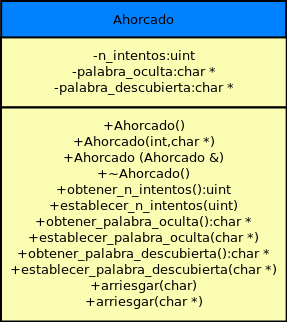
\includegraphics[width=0.45\textwidth]{Ahorcado_UML.png}
  \caption{Diseño UML de la clase Ahorcado}
  \label{fig:disenio}
\end{figure}

\end{document}
